\documentclass[12pt]{article}
\usepackage[pdftex]{graphicx}
\usepackage{url}
\usepackage{setspace}
\usepackage{makeidx}
\usepackage[utf8]{inputenc}
\usepackage{fancyhdr}
\usepackage{layout}
\usepackage{float}
\usepackage{caption}
\usepackage{titlesec}
\usepackage{graphicx}
\usepackage[a4paper,pdftex]{geometry}	% Use A4 paper margins
\usepackage[english]{babel}
\usepackage{xcolor} % Required for specifying custom colors
\usepackage{fix-cm} % Allows increasing the font size of specific fonts beyond LaTeX default specifications
\usepackage{amssymb}
\usepackage{amsthm}
\usepackage{amsmath}
\usepackage{hyperref}
\hypersetup{
    colorlinks,
    citecolor=black,
    filecolor=black,
    linkcolor=black,
    urlcolor=black
}

\DeclareGraphicsExtensions{.pdf,.png,.jpg}

\setlength{\oddsidemargin}{0mm} % Adjust margins to center the colored title box
\setlength{\evensidemargin}{0mm} % Margins on even pages - only necessary if adding more content to this template

\renewcommand{\thesection}{\arabic{section}} %Section numbering
\renewcommand{\thesubsection}{\thesection.\arabic{subsection}} %Subsection numbering

\setlength{\voffset}{-1.2cm}
\setlength{\textheight}{650pt}
\setlength{\parindent}{0pt}
\renewcommand{\baselinestretch}{1.5}
\definecolor{grey}{rgb}{1.0,1.0,0.95} % Color of the box surrounding the title - these values can be changed to give the box a different color	

\pagestyle{fancy}
\fancyhf{}
\lhead{A Fireball for Your Friends}
\rhead{Game Design Document: Part \thepart}
\rfoot{\thepage}

\newcommand*\cleartoleftpage{%
  \clearpage
  \ifodd\value{page}\hbox{}\newpage\fi
}

\newcommand{\sectionbreak}{\clearpage}

\makeindex

\begin{document}

\pagestyle{empty} % Remove page numbering on this page

%----------------------------------------------------------------------------------------
%	TITLE SECTION
%----------------------------------------------------------------------------------------

\colorbox{grey}{
	\parbox[t]{1.0\linewidth}{
		\fontsize{50pt}{30pt}\selectfont % The first argument for fontsize is the font size of the text and the second is the line spacing - you may need to play with these for your particular title
		\vspace*{0.7cm} % Space between the start of the title and the top of the grey box
		
		A Fireball \\ 
		for Your Friends \\ 
        \fontsize{30pt}{34pt}\selectfont
        AI Implementation Details		
		\par
		
		\vspace*{0.4cm} % Space between the end of the title and the bottom of the grey box
	}
}

\vspace*{0.4cm} 
{\large Un \textbf{juego de duelos mágicos multijugador en 3ª persona}}

\begin{spacing}{0.6}
Target: \textit{chicos entre 16-22 años, amantes de los juegos competitivos, mid-core} 

Plataforma: \textit{XBox One, Windows PC}
\end{spacing}


\begin{figure}[h]
    \centering
    
\includegraphics[width=0.6\textwidth]{fireball}
\end{figure}

\vfill % Space between the title box and author information

{\centering \hfill \copyright 2018 Pedro Montoto García} \\

%----------------------------------------------------------------------------------------

\clearpage

\setlength{\voffset}{0cm}
\setlength{\parindent}{1cm}
\setcounter{page}{1}

\section{AI Agents}

Describimos aquí los componentes de IA desarrollados.

\subsection{Enemy Example}

El \textit{\emph{EnemyExampleBP}} es un \textit{\emph{MainPlayerBP}} controlado por IA, usando \textit{\emph{EnemyExampleAIControllerBP}} con el árbol de comportamiento \textit{\emph{BTEnemyExample}}. La única modificación que tiene consiste en que su regeneración de maná es ligeramente más alta, para ayudar a mantener la presión sobre el jugador.

\begin{figure}[h]
    \centering
    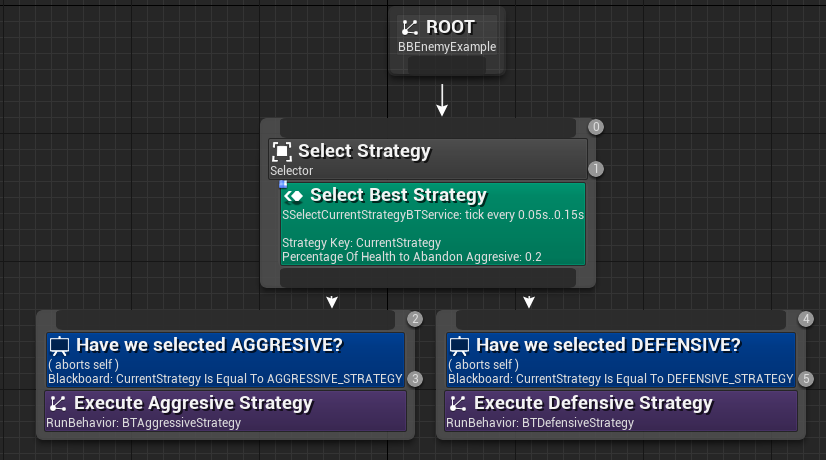
\includegraphics[width=1\textwidth]{base_behavior_tree}
\end{figure}

En la raíz del arbol de comportamientos seleccionamos entre una estrategia agresiva o defensiva (implementadas cada una en su propio sub-árbol). Se escoge estrategia defensiva, por el momento, si el agente tiene menos de un 20\% de su salud total, y agresiva en caso contrario.

\begin{figure}[H]
    \centering
    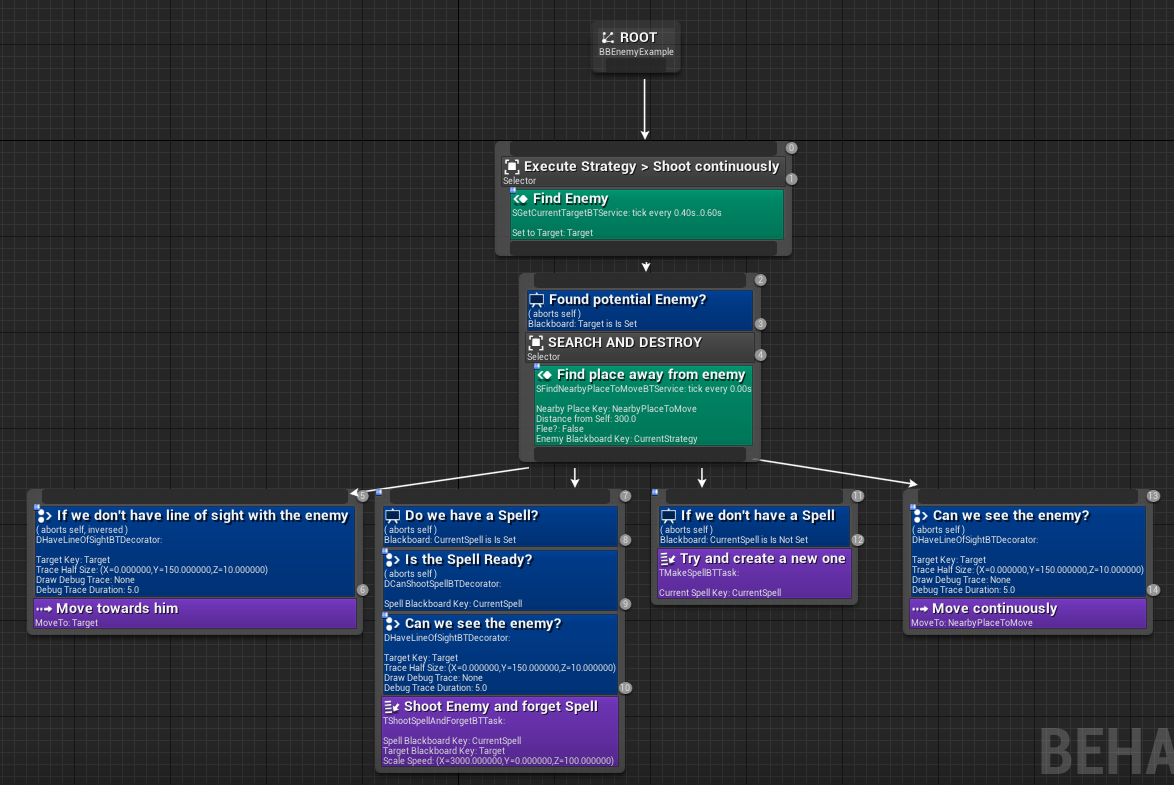
\includegraphics[width=1\textwidth]{aggresive_behavior_tree}
\end{figure}

La estrategia agresiva consiste en mantener una presión constante sobre el enemigo sin dejarle respirar. Para ello se ejecutan, según prioridad, estas tareas:

\begin{enumerate}
	\item Si no podemos ver al enemigo (utilizando un raytrace rectangular, para dejar espacio para los disparos), nos movemos hacia él.
	\item Si no tenemos un hechizo preparado creamos uno nuevo y lo mantenemos
	\item Si podemos ver al enemigo
	\begin{enumerate}
		\item Disparamos continuamente
		\item Nos movemos continuamente para no ser alcanzados
	\end{enumerate}
\end{enumerate}

\begin{figure}[H]
    \centering
    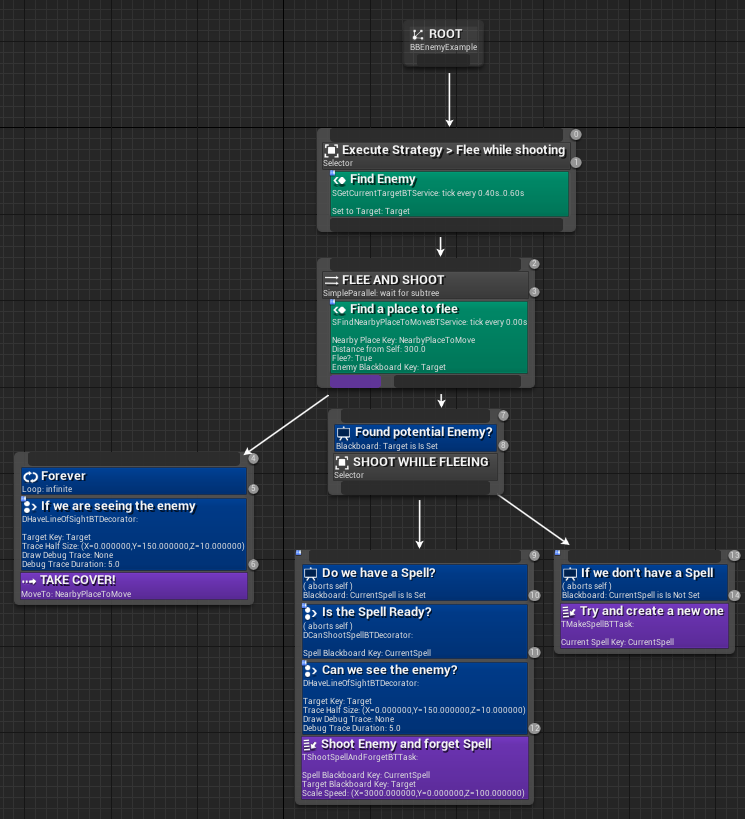
\includegraphics[width=1\textwidth]{defensive_behavior_tree}
\end{figure}

La estrategia defensiva consiste en mantenerse a cubierto, lanzando hechizos mientras se huye para rechazar al enemigo si éste está a la vista.

Añadimos como detalles de implementación que no son completamente intuitivos a primera vista.

\begin{itemize}
	\item La implementación del nodo \textit{\emph{DHaveLineOfSightBTDecorator}} que determina si hay línea de visión entre 2 jugadores no se implementa con un raytrace simple, sino con un box trace, para permitir dejar espacio para disparar los hechizos que siguen a los jugadores con un offset (con \textit{FollowerCBP}).
	\item La implementación del nodo \textit{\emph{SFindNearbyPlaceToMoveBTService}}, que decide el siguiente punto del mapa al que moverse (para no parar de moverse), sigue el siguiente esquema:
	\begin{figure}[H]
	    \centering
	    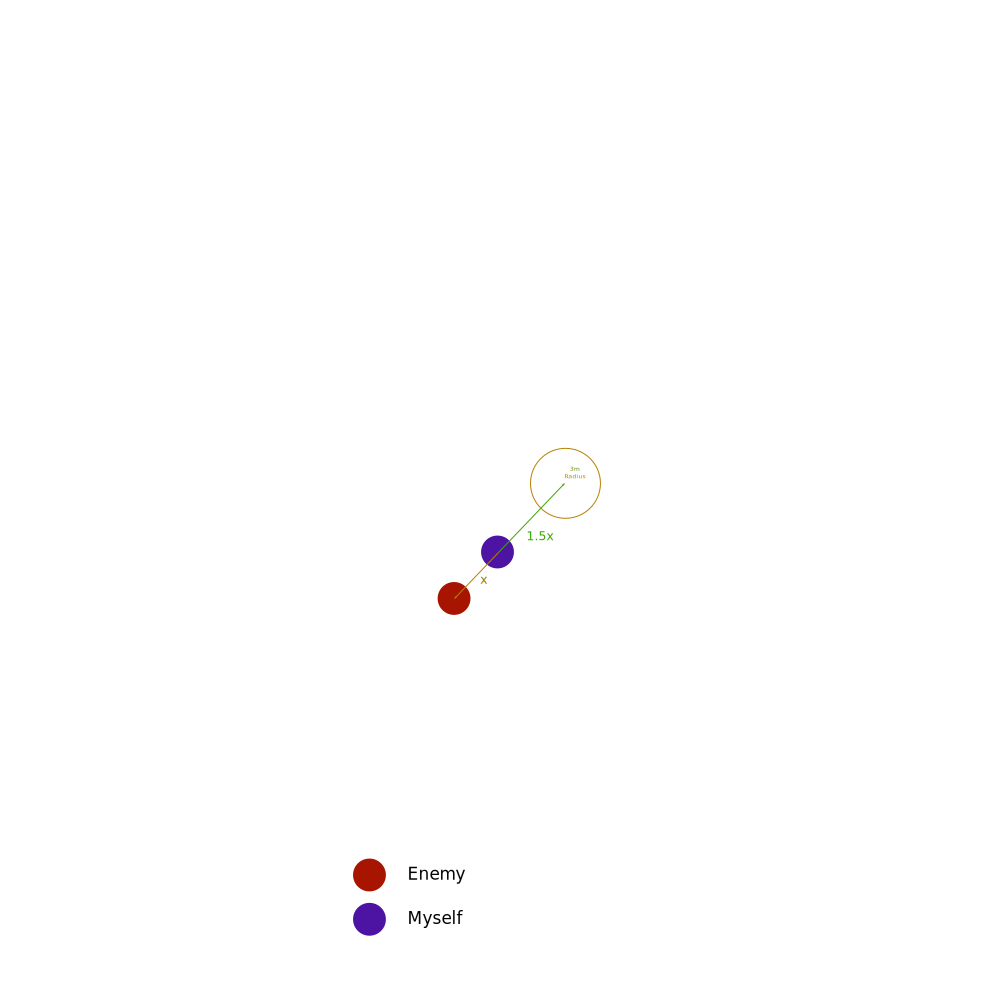
\includegraphics[width=1\textwidth]{positioning_scheme}
		\captionsetup{labelformat=empty}
	    \caption{Se selecciona un punto aleatorio dentro del círculo de 3 metros para ser el siguiente punto al que moverse, a partir de la posición del enemigo. Si no se está huyendo símplemente se considera $x = 0$ en el esquema anterior, i.e. alrededor del propio agente.}
	\end{figure}
\end{itemize}

\begin{figure}[h]
    \centering
    
\includegraphics[width=0.6\textwidth]{fireball}
\end{figure}

\vfill

\end{document}
